\documentclass[xcolor=pdftex,dvipsnames,table,aspectratio=169]{beamer}
%\documentclass[xcolor=pdftex,dvipsnames,table,handout,aspectratio=169]{beamer}

%\setbeameroption{show notes}

\usepackage{bm,graphicx,multirow,amsmath,tikz} %fancybox,
\usepackage{color}%,textpos}
\usepackage[round]{natbib}
\usepackage[normalem]{ulem}
\usepackage{hyperref}
\usepackage{lastpage}
\usepackage{array}
\usepackage{color}
\usepackage{framed}
\usepackage{hyperref}

% Define Western colours
\definecolor{western}{rgb}{.306,.152,.524}
\definecolor{westerngray}{rgb}{.512,.508,.524}

%% Define BEAMER colours
\setbeamercolor{frametitle}{bg=western,fg=white}
\setbeamercolor{framesubtitle}{bg=western,fg=black}
\setbeamercolor{title}{fg=white,bg=western}
\setbeamercolor{author}{fg=white,bg=western}
\setbeamercolor{institute}{fg=white,bg=western}
\setbeamercolor{date}{fg=white,bg=western}

%% Set BEAMER fonts
\setbeamerfont{title}{shape=\bf}
\setbeamerfont{frametitle}{shape=\sc,size=\Large}
\setbeamerfont{framesubtitle}{shape=\sc,size=\Large}
\setbeamerfont{footline}{shape=\sc}

%% Define BEAMER toc
\setbeamercolor{section in toc}{fg=western}
\setbeamercolor{subsection in toc}{fg=westerngray}
\setbeamertemplate{sections/subsections in toc}[ball]

%% Define BEAMER background
\setbeamercolor{background canvas}{bg=white}

%% Define BEAMER footer
\setbeamertemplate{navigation symbols}{}
\setbeamercolor{footline}{fg=white,bg=western}
\setbeamertemplate{footline}{%
  \begin{beamercolorbox}[wd=\paperwidth]{footline}
    \vskip5pt

    \raisebox{.05in}{
      \scriptsize{\bf \insertshorttitle}
    }
    \hfill
    \raisebox{.05in}{
      \scriptsize{\bf \insertframenumber/\inserttotalframenumber} 
    }
    \hspace{5pt}

    \vskip5pt
  \end{beamercolorbox}
}

%% Define BLOCK environment
\setbeamercolor{block title}{fg=western}
\setbeamerfont{block title}{series=\bfseries}

%% Define ENUMERATE and ITEMIZE environements
\setbeamertemplate{itemize item}[ball]
\setbeamertemplate{enumerate item}[ball]
\setbeamercolor{item projected}{bg=western}

%% Define BEAMER toc
\setbeamercolor{sections/subsections in toc}{fg=blue!75}
\setbeamertemplate{sections/subsections in toc}[ball]

% %% Define SECTION openings
% \AtBeginSection[]{
%   \begin{frame}{\insertshorttitle}
%     \tableofcontents[currentsection,subsectionstyle=hide/hide/hide]
    
%   \end{frame}
% }

%% Define BEAMER frametitle
\addtobeamertemplate{frametitle}{
   \let\insertframetitle\insertsectionhead}{}
\addtobeamertemplate{frametitle}{
   \let\insertframesubtitle\insertsubsectionhead}{}


\makeatletter
  \CheckCommand*\beamer@checkframetitle{\@ifnextchar\bgroup\beamer@inlineframetitle{}}
  \renewcommand*\beamer@checkframetitle{\global\let\beamer@frametitle\relax\@ifnextchar\bgroup\beamer@inlineframetitle{}}
\makeatother

% Define counters for example and exercise
\newcounter{example}
\newcounter{exercise}

% Define example and exercise commands
\renewcommand{\example}
{\stepcounter{example}Example \lecturenum.\arabic{example}}
\newcommand{\examplectd}
{Example \lecturenum.\arabic{example}\ ctd}
\newcommand{\exercise}
{\stepcounter{exercise}Exercise \lecturenum.\arabic{exercise}}
\newcommand{\exercisectd}
{Exercise \lecturenum.\arabic{exercise}\ ctd}

\newcommand{\lecturenum}{17}

\title[SS2857]{Probability and Statistics I}
\subtitle{\lecturenum. The Gamma Distribution and Its Relatives}

\date{}

%% Add logo
% \titlegraphic{\includegraphics[height=2cm]{../uwo_logo_reversed}}

%% Initialize R



\begin{document}

{
\setbeamertemplate{footline}{}
\setbeamercolor{background canvas}{bg=western}

\begin{frame}
  \addtocounter{framenumber}{-1}

  \maketitle
\end{frame}
}

\section{Review}
\begin{frame}<handout:0>

  Suppose that $X \sim \mbox{Normal}(50, 25)$.

  \bigskip
  
  \begin{enumerate}
  \item TRUE or FALSE: $\frac{X-50}{25} \sim \mbox{Normal}(0,1)$.
  \item Multiple choice: $P(a < X < b) \approx .95$ if
    \begin{tabular}{ll}
      a) $a=25$, $b=75$ & b) $a=45$, $b=55$\\
      c) $a=0$, $b=100$ & d) $a=40$, $b=50$
    \end{tabular}
  \item Multiple choice: The pdf of $X$ is
    \begin{tabular}{ll}
      a) Symmetric about 50 &
                               b) Symmetric about 25\\
      c) Left skewed  &
                       d) Right skewed\\
    \end{tabular}
  \item Multiple choice: The support of $X$ is
    \begin{tabular}{ll}
      a) All of $\mathbb R$. &
                               b) The positive real line.\\
      c) The interval (35,65). &
                       d) The non-negative integers.
    \end{tabular}
    

  \end{enumerate}
  
  
\end{frame}

\section{}

\begin{frame}
  
  \begin{center}
    \Large{\textbf{4.3 The Gamma Distribution and Its Relatives}}
  \end{center}
  
  \bigskip
  
  
\end{frame}

\begin{frame}
  
  \begin{center}
    \Large{\textbf{4.3a The Gamma Distribution}}
  \end{center}
  
  \bigskip
  
  \begin{center}
    
\includegraphics[height=.5\textheight]{figure/weather-vancouver}
  \end{center}
\end{frame}

\section{The Gamma Distribution}

\begin{frame}
  \begin{block}{Gamma Distribution}
    A continuous random variable, $X$, has a gamma distribution if the pdf of $X$ is
    \[
      f(x)=\frac{1}{\beta^\alpha\Gamma(\alpha)}x^{\alpha-1}e^{-x/\beta},\quad x \geq 0.
    \]
    Mathematically, we write $X \sim \mbox{Gamma}(\alpha,\beta)$.
  \end{block}

 \begin{block}{Properties}
%    \begin{columns}
%      \begin{column}{.5\textwidth}
        \begin{itemize}
        \item CDF: No closed form

%        \item MGF: $M_X(t)=\frac{1}{(1-\beta t)^{\alpha}}$

        \item Mean: $E(X)=\alpha\beta$
%        \end{itemize}
%      \end{column}
      
%      \begin{column}{.5\textwidth}
%        \begin{itemize}
        \item Variance: $V(X)=\alpha\beta^2$

%        \item Skewness: $\frac{2}{\sqrt{\alpha}}$

        \end{itemize}
%      \end{column}
%    \end{columns}
  \end{block}  
\end{frame}

\begin{frame}
  \begin{block}{The Gamma Function}
    For $\alpha>0$ the gamma function is defined as 
    \[
      \Gamma(\alpha)=\int_0^\infty x^{\alpha-1}e^{-x}~dx.
    \]
    
    \bigskip
    
    \textbf{Properties}
    \begin{enumerate}
    \item $\Gamma(1)=1$
    \item For any $\alpha>0$, $\Gamma(\alpha)=(\alpha-1)\Gamma(\alpha-1)$
    \item For any positive integer, $n$, $\Gamma(n)=(n-1)n\Gamma(n-1)=(n-1)!$
    \item $\Gamma(1/2)=\sqrt{\pi}$. 
    \end{enumerate}
  \end{block}
\end{frame}

\begin{frame}

\begin{block}{Calculator}

\begin{center}
\url{https://homepage.divms.uiowa.edu/~mbognar/applets/gamma.html}
\end{center}

\bigskip

Note: we are using the \textit{scale} parameterization.
\end{block}
\end{frame}





\begin{frame}
  
  \begin{block}{\example: The Gamma Distribution}
    It rained/snowed/precipitated in London on 179 days in 2018. The following histogram summarizes the total millimeters of precipitation on these days.

    \begin{center}
      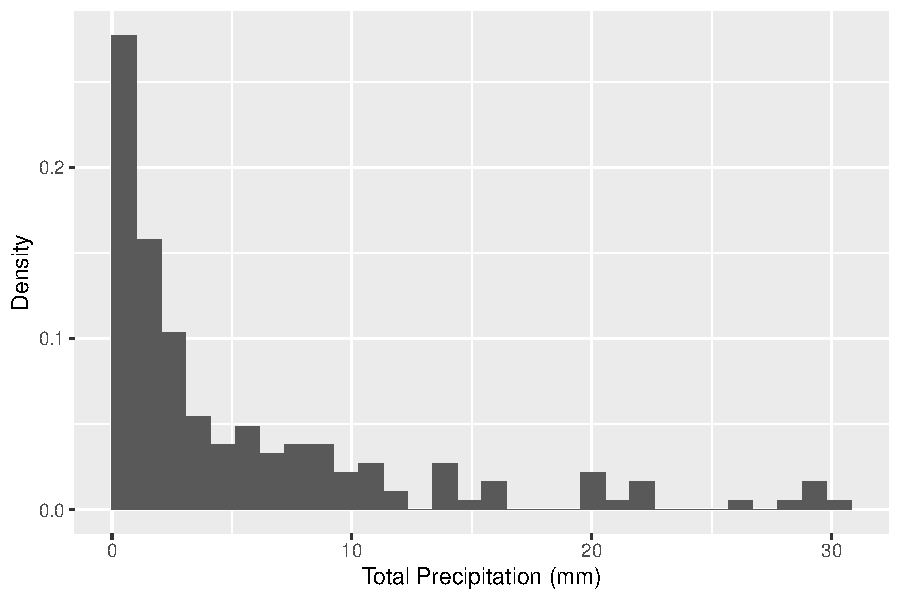
\includegraphics[height=.6\textheight]{figure/gamma1-1}
    \end{center}

  \end{block}
\end{frame}

\begin{frame}
  \begin{block}{\examplectd: The Gamma Distribution}
    It rained/snowed/precipitated in London on 179 days in 2018. The following histogram summarizes the total millimeters of precipitation on these days.

    This distribution is well modeled by the gamma distribution with parameters $\alpha=0.628$ and $\beta=8.662$. 
    
    \begin{center}
      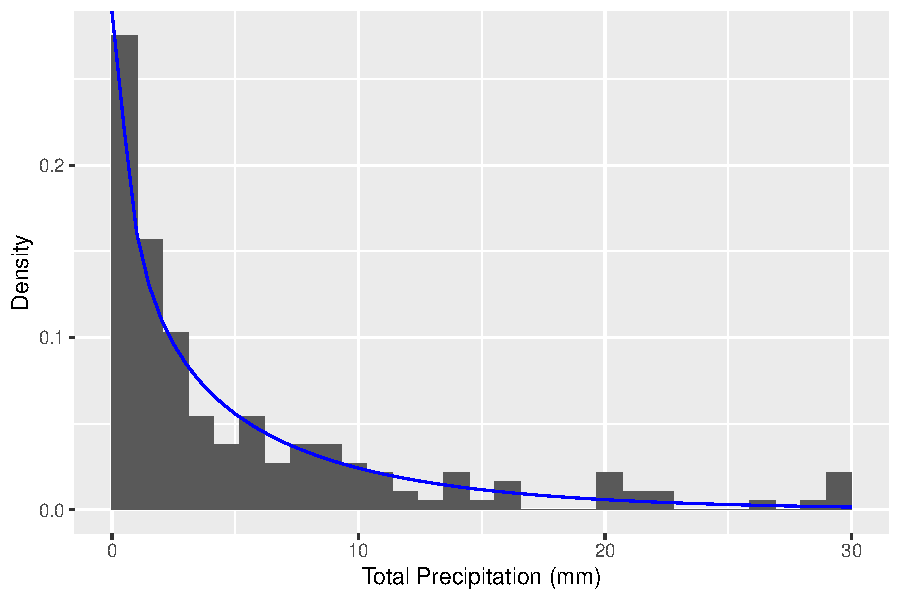
\includegraphics[height=.5\textheight]{figure/gamma1-2}
    \end{center}

  \end{block}
\end{frame}

\begin{frame}
  \begin{block}{\examplectd: The Gamma Distribution}
    Let $X$ denote the total amount of precipitation on a randomly selected rainy day in London. Suppose that
    \[
      X \sim \mbox{Gamma}(0.628,8.662).
    \]

    \begin{enumerate}[a)]
    \item What is the pdf of $X$?
    \item What are the mean and variance?
    \item What is the probability that the total precipitation is more than 10~mm given that it rains at all?
    \end{enumerate}
    
  \end{block}
\end{frame}

\section{\invisible{Hello}}

\begin{frame}
  
  \begin{center}
    \Large{\textbf{4.3b The Exponential Distribution}}
  \end{center}
  
  \bigskip
  
  \begin{center}
    
\includegraphics[height=.5\textheight]{figure/radioactive}
  \end{center}
\end{frame}

\section{The Exponential Distribution}

\begin{frame}
  \begin{block}{Exponential Distribution}
    If $T \sim \mbox{Gamma}(1,\lambda^{-1})$ then we say that $T$ follows an exponential distribution with rate $\lambda$:
    \[
      T \sim \mbox{Exponential}(\lambda).
    \]
    The pdf of the exponential distribution is
    \[
      f(t)=\lambda e^{-\lambda t},\quad t > 0.
    \]
  \end{block}

  \vspace{-.1in}
  
  \begin{block}{Properties}
%    \begin{columns}
%      \begin{column}{.5\textwidth}
        \begin{itemize}
        \item CDF: $F(t)=1-e^{-\lambda x}, \quad t > 0$

%        \item MGF: $M_X(t)=\frac{\lambda}{\lambda-t}$

        \item Mean: $E(t)=\lambda^{-1}$
%        \end{itemize}
%      \end{column}
      
%      \begin{column}{.5\textwidth}
%        \begin{itemize}
        \item Variance: $V(t)=\lambda^{-2}$

%        \item Skewness: 2

        \end{itemize}
%      \end{column}
%    \end{columns}
  \end{block} 
\end{frame}

\begin{frame}

  \begin{block}{Memoryless Property}
  If $T \sim \mbox{Exponential}(\lambda)$ then
      \[
        T-t_0|T>t_0 \sim \mbox{Exponential}(\lambda) 
      \]
  for any $t_0 > 0$. 
  \end{block}
\end{frame}

\begin{frame}
  \begin{block}{\example: The Exponential Distribution}
    Radioactive decay is well modelled by the exponential distribution. Uranium-235 has a half-life of 703,800,000 years. Let $T$ be time in billions of years to decay of a single atom of Uranium-235.

    \bigskip
    
    \begin{enumerate}[a)]
    \item What is the pdf of $T$?
    \item What are the mean and variance of $T$?
    \item What is the probability that $T<1$?
    \item What is the probability that $T>2$ given $T>1$?
    \item What is the probability that $T>100,001$ given $T>100,000$?
     \end{enumerate}
  \end{block}
\end{frame}




\begin{frame}
  \begin{block}{\examplectd}
    \begin{center}
      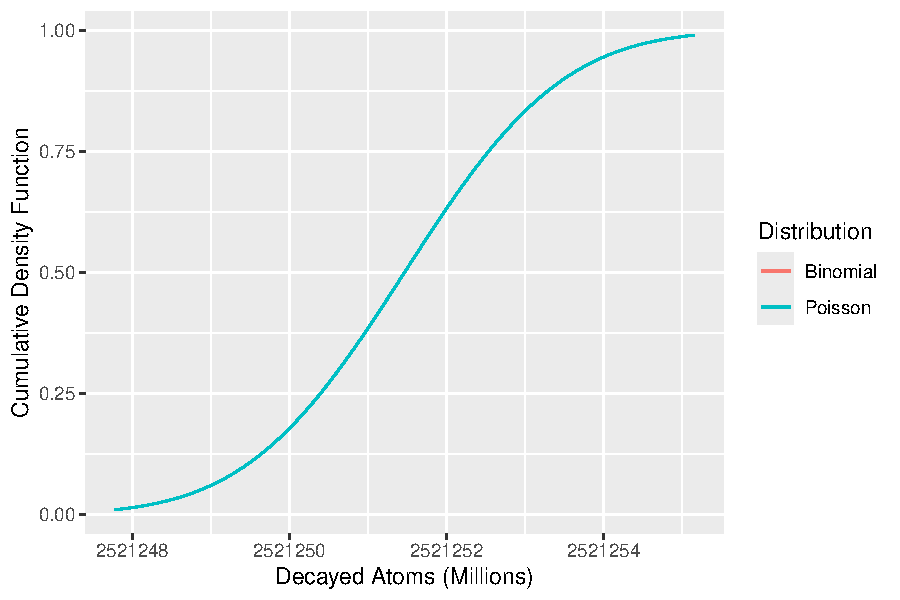
\includegraphics[height=.75\textheight]{figure/exercise2-1}
    \end{center}
  \end{block}
\end{frame}

\begin{frame}
  \begin{block}{Connection to Poisson Process}
    Suppose that we are modelling a Poisson process so that if $X_t$ represents the number of events occurring in any time interval of length $t>0$ then
    \[
      X_t \sim \mbox{Poisson}(\lambda t).
    \]

    \bigskip

    Then the time between any two events follows an exponential distribution with rate $\lambda$. I.e., if the $r^{th}$ event occurs at $T_r$ and the $(r+1)^{st}$ at $T_{r+1}$ then
    \[
      T_{r+1}-T_r \sim \mbox{Exponential}(\lambda).
    \]
    
  \end{block}
\end{frame}

\section{\invisible{Hello}}

\begin{frame}
  \frametitle{\invisible{Hello}}
  
  \begin{center}
    \Large{\textbf{4.3c The Chi-Squared Distribution}}
  \end{center}
  
  \bigskip
  
\end{frame}

\section{The Chi-Squared Distribution}

\begin{frame}
  \begin{block}{Chi-Squared Distribution}
    If $X \sim \mbox{Gamma}(\nu/2,2)$ then we say that $X$ follows a chi-squared distribution with $\nu$ degrees of freedom:
    \[
      X \sim \chi^2_\nu.
    \]
    The pdf of the chi-squared distribution is
    \[
      f(x)=\frac{1}{2^{\nu/2}\Gamma(\nu/2)}x^{(\nu/2)-1}e^{-x/2},\quad x \geq 0.
    \]
  \end{block}

  \vspace{-.1in}
  
  \begin{block}{Properties}
%    \begin{scriptsize}
%    \begin{columns}
%      \begin{column}{.5\textwidth}
        \begin{itemize}
        \item CDF: No closed form

        \item MGF: $M_X(t)=\frac{1}{(1-2t)^{\nu/2}}$
          
        \item Mean: $E(X)=\nu$
%        \end{itemize}
%      \end{column}
      
%      \begin{column}{.5\textwidth}
%        \begin{itemize}
        \item Variance: $V(X)=2\nu$

%        \item Skewness: $\sqrt{\frac{8}{\nu}}$

%        \item Excess Kurtosis: $\frac{12}{\nu}$
        \end{itemize}
%      \end{column}
%    \end{columns}
%  \end{scriptsize}
\end{block}
\end{frame}

\begin{frame}

\begin{block}{Calculator}

\begin{center}
\url{https://stattrek.com/online-calculator/chi-square}
\end{center}
\end{block}
\end{frame}

\begin{frame}
  \begin{block}{Alternative Derivation ($\nu = 1$)}
    Suppose that $Z$ is a standard normal random variable,
    \[
      Z \sim \mbox{Normal}(0,1)
    \]
    Then $X$ 
    \[
      X=Z^2 \sim \mbox{Chi-Squared}(1) \mbox{ or } X \sim \chi^2_1.
    \]
  \end{block}
\end{frame}

\begin{frame}
  \begin{block}{Alternative Derivation ($\nu \geq 1$)}
    More generally, if $Z_1,\ldots,Z_\nu$ are all independent standard normal random variables,
    \[
      Z_i \sim \mbox{Normal}(0,1), \quad i=1,\ldots,\nu
    \]
    then
    \[
      X=\sum_{i=1}^\nu Z_i^2 \sim \mbox{Chi-Squared}(\nu) \mbox{ or } X \sim \chi^2_\nu.
    \]
    
  \end{block}
\end{frame}

\begin{frame}

  \begin{block}{\example}
    Suppose that $Z \sim \mbox{Normal}(0,1)$ and $X \sim \chi^2_1$.

    \bigskip

    Confirm that
    \[
      P(Z^2 \leq 2) = P(X \leq 2).
    \]
    
  \end{block}
\end{frame}
\section{\invisible{Hello}}

\begin{frame}
  
  \begin{center}
    \Large{\textbf{Further Comments}}
  \end{center}
  
  \bigskip
  
  % \only<1>{
  %   \begin{center}
  %     
\includegraphics[height=.5\textheight]{zurg}
  %   \end{center}
  % }
\end{frame}

\section{Final Comments}

\begin{frame}
  \begin{block}{Gamma Distribution}
    \begin{itemize}
    \item Highly flexible model for positive random variables.
    \end{itemize}
  \end{block}

  \pause
  
  \begin{block}{Exponential Distribution}
    \begin{itemize}
    \item Restricted case of gamma ($\alpha=1$).
    \item Satisfies the memory-less property
    \item Models waiting times in a Poisson process.
    \end{itemize}
  \end{block}

  \pause
  
  \begin{block}{Chi-Squared}
    \begin{itemize}
    \item Essential to statistical inference and hypothesis testing.
    \end{itemize}
  \end{block}
\end{frame}

\begin{frame}<handout:0>
  \begin{center}
    \Huge{\textbf{Questions?}}
  \end{center}
\end{frame}

\begin{frame}

\begin{block}{\exercise}

In a Poisson process with rate $\lambda$, the time from one event to the next event, $T$, is exponentially distributed with mean $1/\lambda$. Let $T_k$ denote the time from one event until the $k$-th following event. It turns out that $T_k$ follows a gamma distribution with parameters $\alpha = k$ and $\beta=1/\lambda$. 

\begin{enumerate}[a)]
\item Suppose that $\lambda=.1$ events per second. What are the mean and variance of $T_5$?
\item What is the probability that the $5$-th event occurs after 60 seconds?
\item Compare the the 5-th, 50-th, and 95-th percentiles of $T_5$ and of a normal random variable with the same mean and variance.
\item Repeat the previous step for $T_25$, $T_50$, and $T_100$. Plot the ratio of the percentiles of the two distributions vs $k$. What happens?
\end{enumerate}
\end{block}

\end{frame}
\end{document}
